%\documentclass{beamer}
\documentclass[RawSienna,dvipsnames]{beamer}

%%% Dichiarazione dei pacchetti standard.
\usepackage[italian]{babel}
\usepackage[utf8x]{inputenc}
\usepackage{eurosym}
%%% Personalizzazione del layout---articolata su cinque livelli.
%\usetheme{split}        % layout complessivo. 
%\usetheme{CambridgeUS}
\usetheme{AnnArbor}
\useinnertheme{rectangles} % layout interno.
\useoutertheme{infolines} % layout esterno.
\setbeamercolor{title}{fg=RawSienna}
\setbeamercolor{frametitle}{fg=RawSienna}
\usecolortheme{crane} % schema di colori.
\usefonttheme{professionalfonts}  % schema dei font.
\setbeamercolor{item}{fg=RawSienna}
% Inutile dire che se volete tutti i default, potete risparmiarvi gli ultimi
% quattro comandi. 
%%% Titolo e autore.
\title{Monolith}
\subtitle{An interactive bubble provider}
\author{Revisione di Accettazione}
%\institute{Gruppo Utilizzatoti Italiani di \TeX}
%\date{\today}
\date{11 Settembre 2017}


\usepackage{listings}
\usepackage{color}
\definecolor{lightgray}{rgb}{.9,.9,.9}
\definecolor{darkgray}{rgb}{.4,.4,.4}
\definecolor{purple}{rgb}{0.65, 0.12, 0.82}

\lstdefinelanguage{JavaScript}{
  keywords={typeof, new, true, false, catch, function, return, null, catch, switch, var, if, in, while, do, else, case, break},
  keywordstyle=\color{blue}\bfseries,
  ndkeywords={class, export, boolean, throw, implements, import, this},
  ndkeywordstyle=\color{darkgray}\bfseries,
  identifierstyle=\color{black},
  sensitive=false,
  comment=[l]{//},
  morecomment=[s]{/*}{*/},
  commentstyle=\color{purple}\ttfamily,
  stringstyle=\color{red}\ttfamily,
  morestring=[b]',
  morestring=[b]"
}

\lstset{
   language=JavaScript,
   backgroundcolor=\color{lightgray},
   extendedchars=true,
   basicstyle=\footnotesize\ttfamily,
   showstringspaces=false,
   showspaces=false,
   numbers=left,
   numberstyle=\footnotesize,
   numbersep=9pt,
   tabsize=2,
   breaklines=true,
   showtabs=false,
   captionpos=b
}



\begin{document}
	
\begin{frame}
	\begin{center}
		
\includegraphics[scale=0.13]{img/obelix.png}
		\qquad\qquad
		
\includegraphics[scale=0.13]{img/monolith.png}
	\end{center}
	\titlepage
\end{frame}


\section[Sommario]{}
\begin{frame}
	\tableofcontents
\end{frame}	

\section{Il gruppo Obelix}
\begin{frame}
	
	\begin{columns}
		\begin{column}{0.2\textwidth}
			
		\end{column}
		
		\begin{column}{0.4\textwidth}
			\begin{itemize}
				\item Emanuele Crespan
				\item Tomas Mali
				\item Silvio Meneguzzo
				\item Nicolò Rigato
				\item Riccardo Saggese
				\item Federica Schifano
			\end{itemize}
		\end{column}
		
		\begin{column}{0.2\textwidth}
			
		\end{column}
	\end{columns}
	
	
\end{frame}

\section{Utilizzo SDK}
\begin{frame}
	\frametitle{Hello Bubble - How to}
%[caption=My Javascript Example]
	\begin{center}
	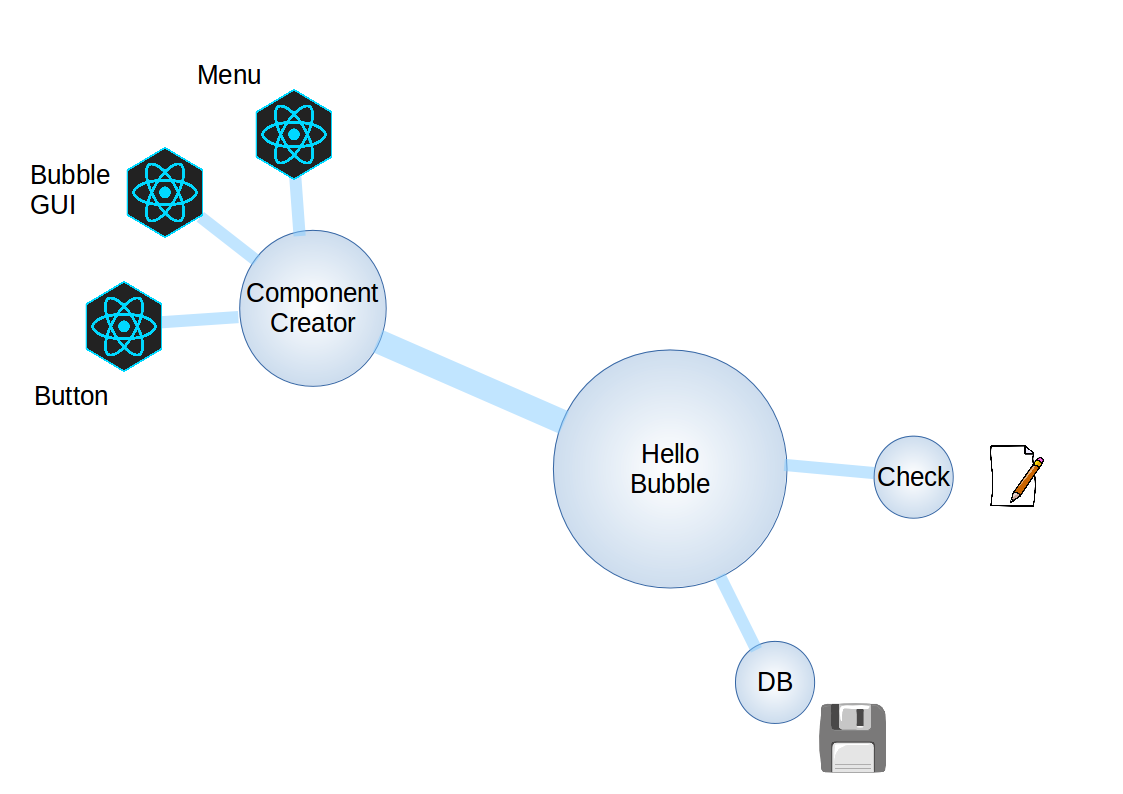
\includegraphics[scale=0.30]{code/bubbleMap.png}
	\end{center}
\end{frame}

\subsection{Hello Bubble - Gui}
\begin{frame}[fragile]
	\frametitle{Bubble Menu}
%[caption=My Javascript Example]
	\begin{center}
	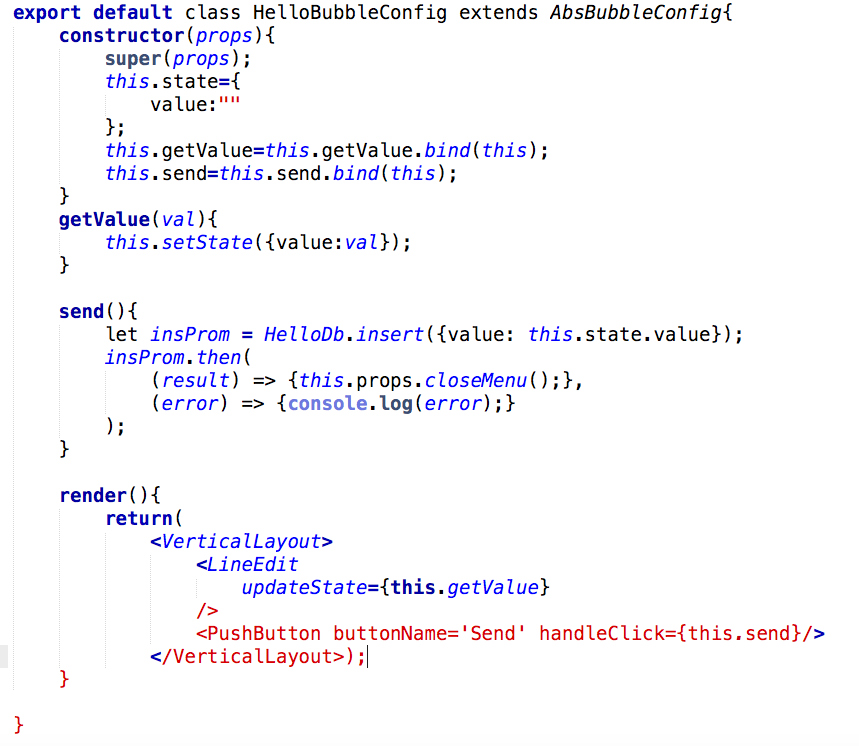
\includegraphics[width=.5\textwidth]{code/hellobubbleconfig.png}
	\vfill
	{
	\vfill
	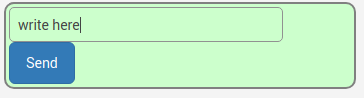
\includegraphics[width=.3\textwidth]{code/config.png}
	\vfill
	}
	\end{center}
\end{frame}

\begin{frame}
	\frametitle{Bubble Button}
%[caption=My Javascript Example]
	\begin{center}
	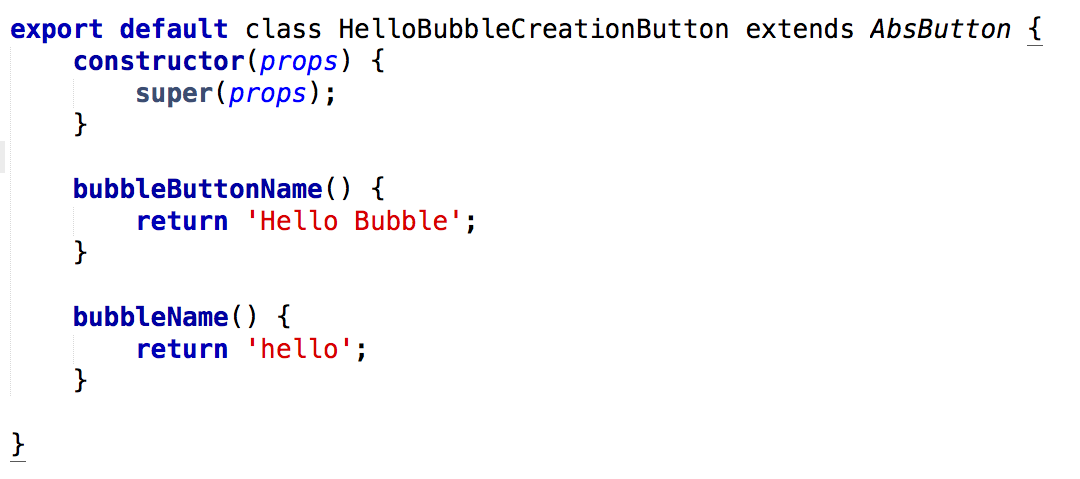
\includegraphics[width=.8\textwidth]{code/hellobubblecreationbutton.png}
	
\includegraphics[width=.3\textwidth]{code/button.png}
	\end{center}
\end{frame}

\begin{frame}
	\frametitle{Bubble Gui}
%[caption=My Javascript Example]
	\begin{center}
	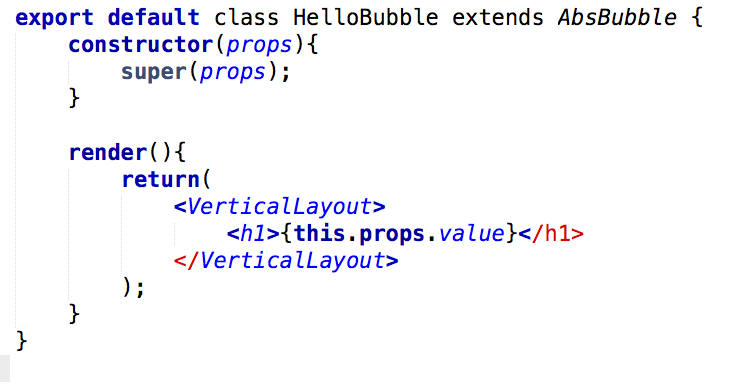
\includegraphics[width=.8\textwidth]{code/hellobubble.png}
	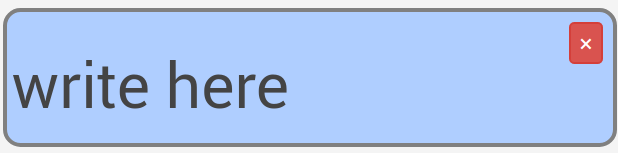
\includegraphics[width=.3\textwidth]{code/bubble.png}
	\end{center}
\end{frame}


\begin{frame}
	\frametitle{Gui managment}
%[caption=My Javascript Example]
	\begin{center}
	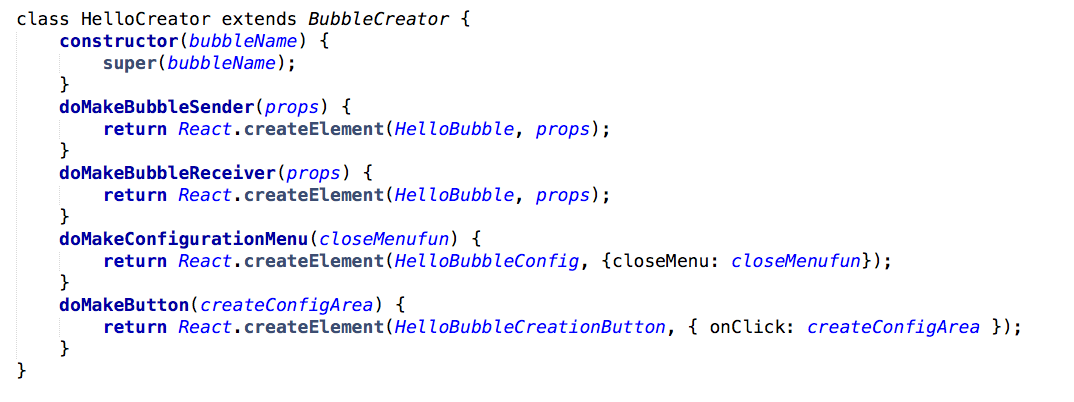
\includegraphics[width=.9\textwidth]{code/hellocreator.png}
	\end{center}
\end{frame}


\subsection{Database and data check}

\begin{frame}
	\frametitle{Database}
%[caption=My Javascript Example]
	\begin{center}
	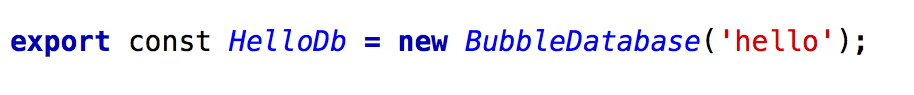
\includegraphics[width=.8\textwidth]{code/helloDb.png}
	\end{center}
\end{frame}

\begin{frame}
	\frametitle{Bubble Check}
%[caption=My Javascript Example]
	\begin{center}
	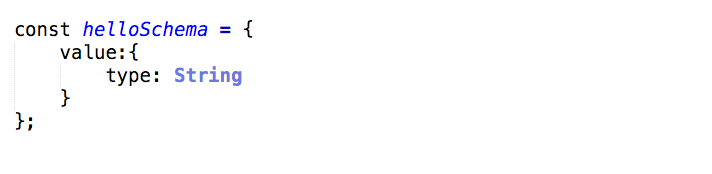
\includegraphics[width=.8\textwidth]{code/hellocheck.png}
	\end{center}
\end{frame}

\section{Bolle Predefinite e Demo}
\subsection{Generali}

\begin{frame}
	\frametitle{Bolle Predefinite e Demo}
	
		
		\begin{columns}
			\begin{column}{0.2\textwidth}
				
			\end{column}
			
			\begin{column}{0.4\textwidth}
				
					 \huge Bolle Predefinite \\
					\begin{center}
					       e \\
					\end{center} 
					\begin{center}
						\huge Demo
					\end{center}
					  
				
				
			\end{column}
			
			\begin{column}{0.2\textwidth}
				
			\end{column}
		\end{columns}
		
		
\end{frame}





\section{Confronto ore preventivate e ore effettive per ruolo}
\begin{frame}
	\frametitle{Confronto ore preventivate e ore effettive per ruolo}	
\begin{center}
	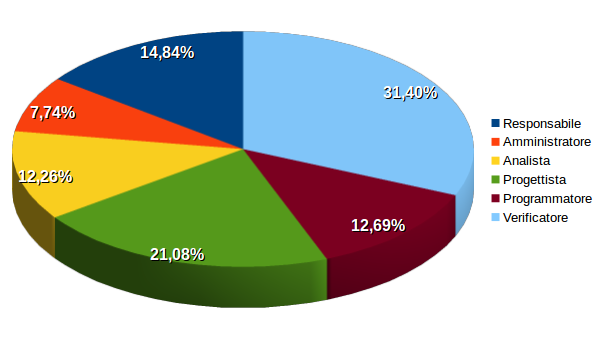
\includegraphics[scale=0.30]{img/orePREVENTIVATEperruolo.png}
	\qquad\qquad
	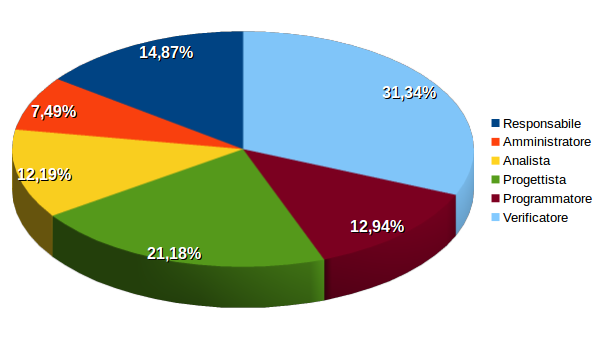
\includegraphics[scale=0.30]{img/oreEFFETTIVEperruolo.png}
\end{center}
	
	
\end{frame}

\section{Confronto costo preventivato e costo effettivo per ruolo}
\begin{frame}
	\frametitle{Confronto costo preventivato e costo effettivo per ruolo}	
	\begin{center}
		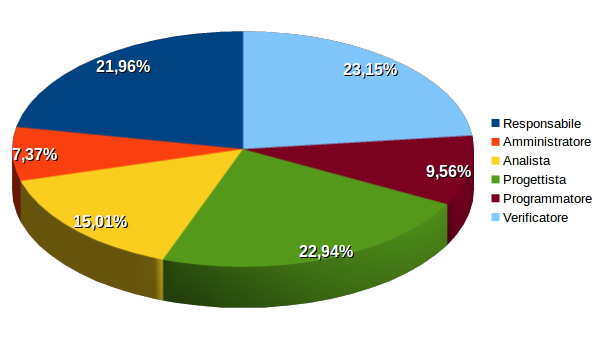
\includegraphics[scale=0.30]{img/costoEFFETTIVOperruolo.png}
		\qquad\qquad
		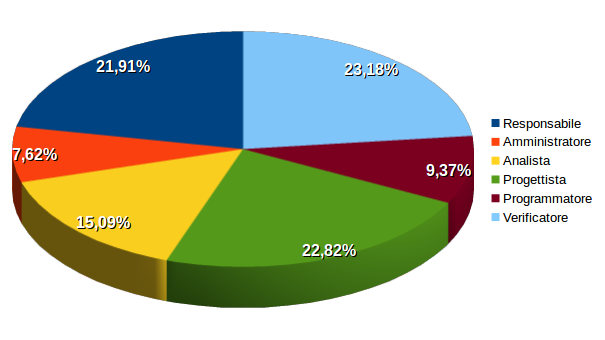
\includegraphics[scale=0.30]{img/costoPREVENTIVATOperruolo.png}
	\end{center}
	
	
\end{frame}


\section{Impegno individuale}
\begin{frame}
	\frametitle{Impegno individuale}	
	\begin{center}
		\centering
		\begin{tabular}{|c|c|c|}
			\hline
			\textbf{Nominativo} & \textbf{Ore preventivate} & \textbf{Ore effettive} \\
			\hline Emanuele Crespan	  & 107  & 107 \\
			\hline Tomas Mali  & 107  & 107  \\
			\hline Silvio Meneguzzo  & 106  & 106  \\
			\hline Nicolò Rigato  & 106  & 108  \\
			\hline Riccardo Saggese   & 107  & 108  \\
			\hline Federica Schifano  & 106  & 108  \\
			\hline
		
			\end{tabular}
		
	\end{center}
	
\end{frame}

\section{Consuntivo}
\begin{frame}
	\frametitle{Consuntivo}

\begin{center}
	\centering
	\begin{tabular}{|c|c|c|}
		\hline
		\textbf{Periodo} & \textbf{Preventivo} & \textbf{Consuntivo} \\
		\hline	\emph{Analisi dei requisiti}  &4425  &4425 \\
		\hline  \emph{Analisi in dettaglio}  &2180  &2165  \\
		\hline  \emph{Progettazione architetturale}  &2997  &2998  \\
		\hline  \emph{Progettazione in dettaglio}  &2830  &2884  \\
		\hline  \emph{Codifica}  &3665  &3680  \\
		\hline  \emph{Validazione}  &2795  &2834  \\
		\hline
		\textbf{Totale} &18892  & 18986  \\
		\hline
		\textbf{Rendicontato} &12287  & \textbf{12381} \\
		\hline
	\end{tabular}
	
\end{center}

\end{frame} 

\end{document}
